\chapter{INTRODUÇÃO}\label{CAP:introducao}
O levantamento feito pelo Instituto Brasileiro de Geografia e Estatísticas (IBGE), em 2013, indicou que 6,2\% da população brasileira tem algum tipo de deficiência \citeonline{IBGE-2013}. O estudo mostra também que 1,3\% da população tem algum tipo de deficiência física. Da população com deficiência física, 46,8\% tem grau intenso ou muito intenso de limitações, nos casos extremos impossibilita a pessoa de realizar as atividades habituais.

O ininterrupto desenvolvimento de novas tecnologias, \textit{softwares} e \textit{hardwares} concebem uma ampla evolução nas estruturas sociais, corporativas e acadêmicas, porém existem áreas ainda pouco exploradas. Entre elas, é possível destacar a concepção das soluções baseadas em Tecnologia Assistiva (TA).

O conceito de TA, apesar de recente, pode ser definido como o conjunto de sistemas, tecnologias e inovações que permitem aumentar as habilidades funcionais de uma pessoa com algum tipo de deficiência e, desta forma, possibilitar sua inclusão. Segundo \citeonline{Bersch}, o objetivo da TA é proporcionar à pessoa com deficiência maior independência, qualidade de vida e inclusão social, através da ampliação de sua comunicação, mobilidade, controle de ambiente, habilidades de aprendizado, trabalho e integração com a família, amigos e sociedade.

O grande desafio de criar as condições necessárias à acessibilidade das Tecnologias da Informação e Comunicação (TICs) por pessoas com deficiência, transformando a interação desses usuários o mais simples possível, é presente dentro da área de Interação Humano-Computador (IHC). É evidente que as características humanas e os estilos de interação são fatores determinantes no modo como é feita a interação com as TICs através das tecnologias.

O desenvolvimento de soluções baseadas em conceitos de TA, usualmente requerem a adoção de técnicas para desenvolvimento tecnológico, provenientes de outras áreas da Ciência da Computação. A Visão Computacional (VC) é a área da ciência que desenvolve teorias e métodos voltados à extração automática de informações úteis contidas em imagens. O objetivo principal é criar e transmitir essas informações às máquinas de forma compreensível \cite{prince2012computer}.


As motivações sociais previamente citadas em conjunção com as áreas de pesquisa de interesse como TA, VC e Processamento Digital de Imagens (PDI), motivou o desenvolvimento do VisiUMouse, uma tecnologia que permite o uso de um computador por pessoas com algum tipo de deficiência física por meio do rastreamento dos movimentos dos olhos através da entrada de vídeo da \textit{webcam}, utilizando os conceitos e premissas da VC. A ideia é disseminar o uso desta tecnologia por qualquer pessoa no mundo por meio da disponibilização desta solução em um repositório público e gratuito \footnote{http://www.visiumouse.com}.

%Visão Computacional é a área da ciência que desenvolve teorias e métodos voltados à extração automática de informações úteis contidas em imagens \cite{prince2012computer}. O objetivo dessa ciência é criar e transmitir essas informações às máquinas de forma compreensível, segundo \citeonline{prince2012computer}.


%% REVDEIA 4: PEÇA PARA ALGUÉM LER TEU TRABALHO EM VOZ ALTA, FACILITA PARA ENCONTRAR OS ERROS , COMO POR EXEMPLO: Restando do trabalho.... esta irei alterar, mas não conseguirei fazer em todo
O restante do trabalho esta organizado da seguinte forma: o Capítulo \ref{CAP2} apresenta a fundamentação teórica necessária para melhor compreensão do trabalho. O Capítulo \ref{CAP3} descreve a Metodologia utilizada ao longo do projeto. O Capítulo \ref{CAP4} apresenta o desenvolvimento da aplicação concebida. O Capítulo \ref{CAP5} apresenta a modelagem do VisiUMouse. O Capítulo \ref{CAP6} expõe os conceitos de Design utilizados,  o Capítulo \ref{CAP6-tecnilogias-utilizadas} apresenta as tecnologias utilizadas no desenvolvimento, o Capítulo \ref{CAP-tecnologia-visiumouse} demonstra como utilizar o VisiUMouse, o Capítulo \ref{CAP7} refere-se aos experimentos de avaliação realizados com o \textit{software} VisiUMouse e faz uma análise de seus resultados e o Capítulo \ref{CAP-consideracoes-finais-trabalhos-futuros} retrata as considerações finais.
%------------------------------------------------------------------


\chapter{FUNDAMENTAÇÃO TEÓRICA E MOTIVAÇÕES}\label{CAP2}
Este Capítulo apresenta os conceitos fundamentais para a fundamentação teórica da leitura desse trabalho, entre os conceitos estão: Tecnologia Assistiva, Visão Computacional, Conceito de Viola-Jones e \textit{Machine Learning}.

A evolução contínua e exponencial das tecnologias possibilitam cada vez mais a criação e melhorias de em vários âmbitos sociais, digitais, acadêmicos e profissionais. Para isso cada pessoa tem acesso a um arsenal de conhecimento imensurável, na \textit{internet}, como a grande quantidade de artigos e pesquisas acadêmicas publicados diariamente e o desenvolvimento e distribuição continuo de \textit{softwares} de código aberto. É evidente o crescimento das possibilidades em todas as áreas de conhecimento com a revolução da informação, representado um novo modelo mundial para todas as pessoas.

\section{TECNOLOGIA ASSISTIVA}\label{Sub:ta-brasil}
Tecnologia Assistiva pode ser considerada como todos os recursos e serviços que contribuem para proporcionar ou ampliar as habilidades funcionais de pessoas com deficiência e consequentemente promover vida independente e inclusão, segundo \citeonline{Bersch}. O termo TA é uma expressão nova, e se refere a um conceito ainda em pleno processo de construção e sistematização. A utilização de recursos de TA, entretanto, remonta aos primórdios da história da humanidade ou até mesmo da pré-história. Qualquer pedaço de pau utilizado como uma bengala improvisada, por exemplo, caracteriza o uso de um recurso de TA. \cite{galvao2009tecnologia-UPPERCASE}.

Especificamente as pessoas com deficiência motora nos membros superiores encontram grande dificuldades em utilizar um computador pessoal, pelo fato de que os dispositivos padrão de interação são controlados basicamente apenas pelo movimento das mãos. Este tipo de deficiência dificulta ou impossibilita a utilização de dispositivos de entrada tradicionais, como o \textit{mouse} e teclado. Para essas pessoas uma tarefa simples de navegar na \textit{internet} se torna um desafio intangível, atenuado apenas pelos poucos, e caros, dispositivos de TA disponíveis no mercado. São menos numerosas ainda, tecnologias que dão suporte a casos onde o usuário tem apenas o controle do movimento da cabeça. 
%Em muitos dos casos de deficiência motora, como por exemplo a ELA (Esclerose Lateral Amiotrófica), deficiência causada por acidente ou paralisia cerebral, essas pessoas possuem as faculdades mentais intactas.


%% REVDEIA 6: DEI UMA REESCRITA NESTE PARÁGRAFO ABAIXO
Estes fatores permitem que essas pessoas interajam com o seu ambiente de outras maneiras não convencionais, com os movimentos ainda restantes, e como os movimentos da cabeça são, os que nestes casos, permanecem funcionais, são movimentos que podem ser explorados para uma possível maneira de interação com o computador. Em casos específicos como este, é necessário haver um dispositivo de TA, focado na entrada de dados, que capte os movimentos da cabeça (como rotação e flexão) e seus elementos, como boca, nariz e olhos, além da fala. 

Considerando estes fatos podemos citar três tipos de entradas, alternativos:

\begin{enumerate}
\item A entrada de vídeo, onde o usuário estará disposto na frente de uma câmera como a \textit{webcam}.

\item A entrada de áudio, onde o usuário vai precisar ter um microfone.

\item E por fim a entrada por meio de contato físico, onde o usuário vai precisar apertar botões ou \textit{switchs}.
\end{enumerate}

% * <tsixav@gmail.com> 2018-04-17T01:00:16.483Z:
% 
% Ainda nessa seção da para falar dos nives de TA: baixo, medio e alto, como o rafa comentou no audio.
% 
% ^.


\section{VISÃO COMPUTACIONAL}\label{Sub:vc}

Visão Computacional (VC) é uma subárea da Inteligência Artificial (IA) que tem como objetivo dar significado as imagens digitais com base em análise. Segundo \citeonline{prince2012computer}, esta análise procura extrair algum conhecimento da representação matricial das imagens. 

São alguns exemplos referentes a área de VC: 
\begin{itemize}
\item A estimativa de segmentação e de movimento.
\item Reconstrução de fotografias para a criação de modelos tridimensionais, como rostos humanos.
\item Análise de segmentação.
\item Reconhecimento de objetos orgânicos e inorgânico.
\item Rastreamento de alvos.
\end{itemize}

Estes desafios tornam-se complexos pelo fato das imagens digitais serem apenas visíveis para o computador, frequentemente são estruturas de dados no formato de matrizes de distribuição de pontos e também pelo fato de não armazenarem informações sobre a cena representada pela imagem, isto é metadados \cite{prince2012computer}.

Um dos grandes desafios da área de VC é a detecção e rastreamento de alvos, principalmente por sua aplicação em sistemas de vigilância de vídeo, análise de atividade humana, monitoramento de tráfego urbano e rural, rastreamento de animais e robótica autônoma. A análise de atividade humana ganha destaque quando possibilita uma automatização ou facilitação de uma atividade, como utilizar o computador todos os dias \cite{alaya2012multipeople-UPPERCASE}.

Visando solucionar os problemas citados anteriormente, a área de VC utiliza de reconhecimento de padrões, aprendizado de máquina (\textit{Machine Learning}), Geometria Projetiva (GP), PDI e teoria dos grafos \cite{prince2012computer}. Isto pode ser comumente visto em aplicações de redes sociais como o reconhecimento de amigos em uma foto do Facebook ou em zoom automático em fotos com muitos rostos. A Figura \ref{fig:exemplo-vc} ilustra um exemplo de múltiplos reconhecimentos de rostos (retângulos verdes) em um mesmo instante.

%[htbp]
\begin{figure}[H]
\caption{Exemplo de aplicação de VC para o reconhecimento de rostos.}
\centering 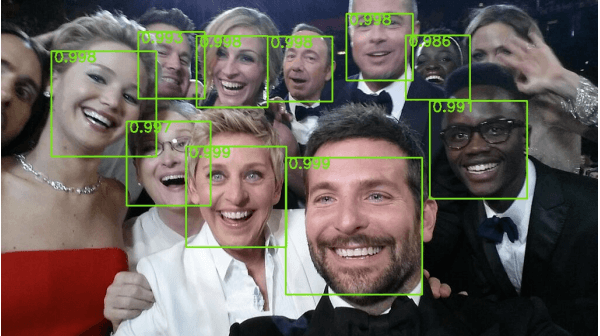
\includegraphics[scale=0.6]{img/figura-1.png}
 
{\fontsize{11}{11}\selectfont \textbf{Fonte:} Elaborada pelo autor.}
\label{fig:exemplo-vc}
\end{figure}

% Considerando três tipos de entrada de dados comuns, como vídeo, áudio e toque é possível analisar que a entrada de vídeo possibilita uma interseção mais natural, considerando que o movimento da cabeça deve ser similar ao movimento da mão quando um usuário sem deficiência utiliza o \textit{mouse}. \textbf{[RCC - Fiquei com dúvida aqui... Estás falando da VC como conceito nesta seção, mas já tenta relacionar com o problema que irás endereçar no projeto. Não sei se este seria o melhor local para fazer esta colocação. Me pareceu fora de contexto, neste ponto. Que acha?]}

Um vídeo pode ser considerado um conjunto de imagens digitais, que é uma representação numérica de uma imagem bidimensional, em forma binária, tornando possível o armazenamento, transferência, processamento ou reprodução por meios eletrônicos. Existe dois tipos de imagens, as imagens de rastreio (ou \textit{raster}) e as imagens do tipo vetorial. \cite{parker2010algorithms-UPPERCASE}. As imagens de rastreio são representadas de forma matricial pelo computador, onde há uma correspondência 'bit-a-bit' da matriz que representa a imagem como o que está sendo reproduzido de fato na tela. A resolução de uma imagem define a sua matriz, então uma imagem de 1024x720 tem 737280 posições em uma matriz. 

As matrizes deste tipo não possuem nem um tipo de dados adicionais como o que existem na imagem ou que tipo de objetos ele representa. A representação e extração destes dados é tarefa da área de VC, que tem como objeto dar significado semântico para imagens digitais através do processamento delas \cite{prince2012computer}. Uma das técnicas para detectar objetos em uma imagem digital é o algoritmo de Viola-Jones. Para a detecção é usado um conjunto de padrões do objeto que se deseja rastrear, para a criação e utilização desses padrões é utilizado \textit{Machine Learning}.

\subsection{Conceito de Viola-Jones}

O algoritmo de Viola-Jones para a identificação de objetos é um algoritmo proposto para o reconhecimento de objetos em imagens digitais, e tem como característica o alto desempenho de processamento e o alto índice de assertividade, podendo chegar até a 99,7\% dependendo do número de etapas treinadas, acurácia do classificador do objeto para qual foi treinado \cite{viola2001rapid}. O algoritmo de Viola-Jones trabalha com algoritmos em cascata que se utiliza de padrões e características chamados de \textit{haar features}. Estas características são organizadas em uma estrutura de árvore em XML (\textit{eXtensible Markup Language}).

\subsection{Machine Learning}

% feito, esta no mesmo nivel só precisava de contextualização
% \textbf{[RCC - essa seção de Machine Learning. Ela está no nível de seção correto (irmã de violaJones)? Porque parece que ficou faltando uma ligação no texto. O ViolaJones ficou bem linkado, essa seção achei meio perdida aqui. Dá uma pensada se ela está no local correto, ou se é necessária]}

\textit{Machine Learning} é utilizada para reconhecer padrões em um grupo de dados, como exemplo podemos citar os padrões que boa parte dos rostos humanos apresentam. Segundo \citeonline{samuel1959some}, podemos definir \textit{Machine Learning} como o campo de estudo que dá aos computadores a habilidade de aprender sem serem explicitamente programados. O aprendizado explora o estudo e construção de algoritmos que podem aprender de seus erros e fazer previsões sobre dados, esses algoritmos operam construindo um modelo a partir de entrada de dados amostrais com o objetivo de fazer previsões ou decisões guiadas pelos dados.

\chapter{METODOLOGIA}\label{CAP3}

Podemos dizer que metodologia é a explicação detalhada e exata de toda ação desenvolvida no (caminho) do trabalho. De acordo com \citeonline{miner2012mapreduce}, é a explicação do tipo de pesquisa, dos instrumentos utilizados, do tempo previsto, da equipe de pesquisadores e da divisão do trabalho, das formas de tabulação e tratamento dos dados, enfim, de tudo aquilo que se utilizou no trabalho de pesquisa.

O objetivo geral do trabalho é desenvolver uma TA com base em VC que permita uma pessoa com deficiência físico motora (principalmente os membros superiores) consiga controlar o seu computador apenas com o movimento da cabeça (usando os olhos como pontos de referência), através da manipulação do movimento e cliques do \textit{mouse}.

Entre os objetivos específicos podemos citar: 
\begin{enumerate}
\item O desenvolvimento do VisiUMouse para multiplataformas.
\item Desenvolvimento do site do VisiUMouse onde será possível fazer o \textit{download} dele de forma gratuita, entre outras funcionalidades.
\item Garantir que os mecanismos de busca dos navegadores modernos achem ele pela busca da palavra 'VisiUMouse'.
\item Desenvolver um instalador.
\item Garantir que o VisiUMouse tenha as principais funcionalidades de um \textit{mouse} tradicional.
\item Criar uma interface de configuração amigável e de utilização simples.
\end{enumerate}

A metodologia utilizada foi exploratória, com o objetivo de investigar e analisar soluções semelhantes ao VisiUMouse, para determinar quais melhorias o VisiUMouse poderia apresentar em relação as TA disponíveis.  
    
\section{TRABALHOS RELACIONADOS}\label{Sub:trabalhos-relacionados}

Existem vários tipos de  \textit{softwares} de TA, e a seguir são apresentados alguns. Parte deles são utilizados para a comunicação com outras pessoas, porém existem outros que tem como objetivo a independência, o qual permite que seus usuários exerçam atividades sozinhos ou com a mínima ajuda possível, ou seja, torna o usuário mais autônomo.

Existem diversos projetos, produtos e estudos em TA, baseados na VC, que utilizam-se de \textit{softwares} para detecção de objetos através de uma \textit{webcam} \cite{ramos2016letras} , \cite{gips2000camera}, \cite{bian2016facial}, \cite{marnik2014blinkmouse}. A detecção dos movimentos nesses projetos é feita através de uma entrada de vídeo que rastreia várias partes do corpo humano, sendo que a mais comum é o rastreamento de movimentos da cabeça (\textit{video-based}). \cite{al2013eye-UPPERCASE}. 

Um dos objetivos de análise desses trabalhos é não depender de dispositivos de alto poder computacional, utilizando Tecnologias disponíveis no próprio computador. Das soluções \textit{video-based} a mais adotada é o \textit{software} CameraMouse \cite{gips2000camera} que frequentemente é usado como base de pesquisas e de comparações, como em Kurauchi \cite{kurauchi2015hmagic}. A seguir são apresentados um resumo de alguns dos \textit{softwares} difundidos no meio.

\subsection{CameraMouse}
O \textit{software} CameraMouse é capaz de capturar o movimento dos olhos ou qualquer outra parte do corpo com que se queira manipular o \textit{mouse} do computador. Ele foi desenvolvido para trabalhar com a plataforma Windows e seu funcionamento se dá através dos recursos do \textit{webcam}. O programa foi desenvolvido para ajudar as pessoas com deficiência e o principal público-alvo deste \textit{software} são as pessoas que não têm controle confiável das mãos, mas que podem executar movimentos com a cabeça \citeonline{gips2000camera}.

Dentre os softwares similares este é o mais semelhante a Tecnologia VisiUMouse, usando dos mesmos conceitos e princípios da VC. A Figura \ref{fig:camera-mouse} apresenta a tela inicial do CameraMouse, o quadrado pequeno na cor verde posicionado no nariz da pessoa representa a área que o usuário selecionou para o \textit{software} rastrear, forçando o usuário estar sempre na mesma posição, podendo apenas mover sua cabeça em inclinar para os lados, forçando o usuário a fazer movimentos espelhados  e assim causando um maior esforço do usuário. O CameraMouse não possibilita usar a inclinação da cabeça para controlar o \textit{mouse}, isto é, para o usuário mover o ponteiro ele preciso imaginar que na tela do computar existe um espelho e que ele deve posicionar o quadrado verde na área que deseja.

\begin{figure}[ht]
 \caption{Tela inicial do Software CameraMouse.} 
\centering 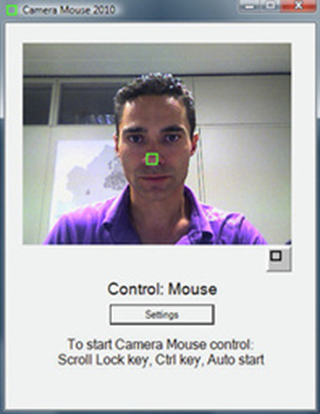
\includegraphics[scale=1]{img/camera-mouse.png}

{\fontsize{11}{11}\selectfont \textbf{Fonte:} Elaborada pelo autor.}
\label{fig:camera-mouse}
\end{figure}

\subsection{HeadDev}

O projeto HeadDev \citeonline{alvesferramentas} é semelhante ao CameraMouse, porém faz o rastreamento apenas dos movimentos da cabeça, não permitindo configurar o objeto que o \textit{software} deve rastrear. Seu funcionamento também utiliza a técnica de espelhamento.

HeadDev é um software gratuito para IHC sem o uso das mãos, cabos, sensores ou outro dispositivo. A interação é feita com uma \textit{webcam} USB padrão, que reconhece os movimentos do rosto. Ele destina-se a pessoas com deficiência motora grave (esclerose lateral amiotrófica, esclerose múltipla, paralisia cerebral, lesão medular e distrofia muscular), porque o sistema só utiliza os movimentos do nariz ou face como ponteiro do \textit{mouse} em um teclado virtual na tela do computador para fazer os eventos de um \textit{mouse}.

\subsection{Facial Mouse}

Facial Mouse é uma interface de IHC para as pessoas com tetraplegia baseada em uma câmera de profundidade de infravermelho monocular. A posição do nariz junto com a boca é detectado para o controle e navegação do cursor do \textit{mouse}. O algoritmo utilizado para rastrear é baseado em uma árvore melhorada de decisão aleatória que é capaz de detectar a informação facial de forma eficiente e com precisão. Com isso é possível uma experiência melhor para o usuário, tornando mais confortável o alcance do movimento do nariz para o movimento do cursor através de uma função não-linear. A câmera de profundidade infravermelha permite o sistema ser independente de iluminação e mudanças de cor tanto no fundo, quanto no rosto humano, o que é uma vantagem crítica sobre as opções baseadas em câmera RGB \citeonline{bian2016facial}.

\subsection{Facial Human-Computer Interface}

Já o \textit{softwares} Facial Human-Computer Interface \citeonline{antunes2016intelligent}, tem como objetivo aplicar o modo de interação feita pelo CameraMouse, refinando a funcionalidade do clique, principalmente nos requisitos de precisão e configuração.

O Facial Human-Computer Interface é um sistema com IHC, que permite uma comunicação mais natural com as máquinas, seu público alvo são pessoas idosas e deficientes. Ele apresenta um sistema baseado em visão e recurso para detecção de piscadas voluntárias longas e interpretação de padrões de piscada para comunicação entre homem e máquina. Complementado pelo mecanismo de detecção de múltiplas piscadas de olho, além disso oferece uma solução completa para a construção de dispositivos de entrada inteligentes com viva-voz. A técnica rastreia utilizando câmeras automáticas que permitem rastrear as características do nariz, sobrancelhas e a posição da cabeça de forma robusta e precisa nas coordenadas 2D e 3D. Esse rastreamento e monitoramento permitem que o usuário forneça dados para a máquina do computador e acesse todo o sistema de uma maneira livre, de acordo com \citeonline{parmar2012facial}. 


\section{OBJETIVO}\label{sub:objeto}

Baseado nos trabalhos relacionados percebe-se a utilização dos conceitos de VC e o uso da OpenCV, com a técnica de espelhamento do movimento e rastreamento da face principalmente. 



\textbf{Nesse contexto o VisiUMouse tem como um dos objetivos implementar uma técnica de movimento alternativa, batizada de Técnica de Zona Neutra e de Movimento (TZNM) \citeonline{xavier2017visiumouse}, com o rastreamento dos olhos para o controle do ponteiro, facilitando uma implementação futura de clique pelo piscar dos olhos e \textit{Eye Tracking}.}


%% REVDEIA 11: AQUI TAMBÉM ACHO QUE DEVERIA IR PARA O CAPÍTULO DO VISIUMOUSE 

\section{VIABILIDADE}\label{Sub:viabilidade}

Com a crescente evolução das áreas de IA é evidente o aumento de ferramentas e estudos que colaboram para a criação e implementação de novas aplicações. Uma subárea da IA que vem ganhando destaque é a VC que tem como foco extrair significado das imagens virtuais com base em análise e estudo de padrões.

Com a evolução da VC possibilitou a criação de novas aplicações, toda atividade humana que tem como base a visão pode ser transformada em uma aplicação de VC. Grandes inovações nas áreas de saúde e Astronomia com a ajuda desta área agora são possíveis. Atualmente é possível utilizar esta área para a busca de estruturas estranhas em imagens de exames de tomografia. 
    
O potencial e a evolução da VC perpetuam o aumento de novos estudo e ferramentas. OpenCV é uma biblioteca grátis e multiplataforma, isto é compatível com múltiplos Sistemas Operacionais e Linguagens de Programação, como Java e C, ela foi desenvolvida pela Intel Corporation, que implementa diversos módulos e cerca de 350 algoritmos de VC, e atualmente está presente em diversos \textit{software} e estudos, tornando as aplicações de VC mais acessíveis.  

Os fatores apresentados manifestam as possibilidades de criação de aplicações com base em VC, grande parte deste cenário é possível graças a biblioteca OpenCV que é uma biblioteca de código aberto e compatível com os principais Sistemas Operacionais e Linguagens de Programação do mercado. Estes fatores determinam a escolha dela e da Linguagem de Programação Java para o desenvolvimento do trabalho. Assim como a maioria das Linguagens de Programação a Java não gera custos.

O trabalho proposto tem como público-alvo pessoas com algum tipo de deficiência motora ou física, que possuem o movimento da cabeça e com a capacidade cerebral preservada.

Os fatores apresentados e a experiência adquirida em outros projetos relacionados com acessibilidade e TA evidenciam aspectos para a viabilidade do trabalho apresentado. Entre as experiências podemos citar a quantidade de usuários com deficiência físico motora no Brasil e na região de Pelotas; de instituições que amparam esses usuários as quais podem ser abordadas diretamente para apresentar o VisiUMouse; que boa parte desses usuários não estão presentes diretamente na sociedade.

\section{METODOLOGIA DE DESENVOLVIMENTO}\label{Sub:metodologia-desenvolvimento}
Para o desenvolvimento desse trabalho foi utilizado o método de Design Centrado no Usuário (DCU), de acordo com \cite{GREENHOUSE2010}, a metodologia DCU não é um estilo de design, mas sim um processo para projetar e desenvolver produtos que se baseiam em informações sobre as pessoas que vão utilizá-las, uso de resultados de pesquisas e dados sobre habilidades cognitivas, capacidades físicas e limitações, necessidades sociais e os requisitos de tarefas com o objetivo de fornecer soluções para aplicações que sejam de acesso universal, independentemente de idade ou habilidade. 

Além disso foi utilizado a Metodologia Ágil SCRUM, nele os projetos são divididos em ciclos chamados de \textit{Sprints}. O \textit{Sprint} representa um \textit{Time Box} dentro do qual um conjunto de atividades deve ser executado. O SCRUM foi utilizado principalmente para organizar a prioridade das \textit{Sprints} relacionadas ao desenvolvimento, para garantir as datas de entrega e a organização do tempo disponível, segundo \citeonline{miner2012mapreduce}.

Para realizar os objetos desse trabalho, todo desenvolvimento do \textit{software} do VisiUMouse foi organizado em 3 ciclos: \textbf{Validação}, \textbf{Experimento} e \textbf{Melhoria}. A \textbf{Validação} foi ciclo inicial da criação da solução e tinha como objetivo validar a solução proposta, para validar foi criado um MVP, que tinha como principal funcionalidade o rastreamento dos olhos e o controle do \textit{mouse}; O \textbf{Experimento} teve como objetivo comprovar seu funcionamento, de uma tecnologia que permite o controle do \textit{mouse} apenas com o movimento da cabeça, além de levantar possíveis melhorias, como um autoajuste dos parâmetros de rastreamento e otimizar os algoritmos de processamento de vídeo; O último ciclo, \textbf{Melhoria},  compreendeu em implementar as melhorias levantadas no ciclo de \textbf{Experimento}, e após disponibilizar uma versão do \textit{software} do VisiUMouse no site oficial 'www.visiumouse.com'.

\chapter{MODELAGEM}\label{CAP5}

Segundo \citeonline{pressman2016engenharia}, a modelagem de \textit{software} é de extrema importância no processo de desenvolvimento pois ajuda a determinar as necessidades de um sistema de informação. Foram utilizados os conceitos de Linguagem de Modelagem Unificada (UML) para a modelagem de diagramas. Através deles foi possível ter uma visão mais refinada do funcionamento do VisiUMouse e possíveis pontos instáveis do projeto.

\section{Diagrama de Caso de Uso}
O Diagrama de Caso de Uso utiliza uma representação simples, descrevendo o comportamento externo do VisiUMouse, apresentando a solução através de uma perspectiva do usuário, demonstrando as funções e funcionalidades disponíveis. Segundo \citeonline{guedes2011uml}, este diagrama é o mais abstrato, flexível e informal, sendo o utilizado com mais frequência na modelagem de sistemas.%, sendo uma base confiável para a modelagem, . 

A Figura \ref{fig:use-case-diagram} mostra o Caso de Uso do VisiUMouse. O diagrama é composto por dois atores. 
\begin{itemize}
\item \textit{Usuário}: ator representando o usuário que vai utilizar o computador apenas com o movimento dos olhos. %, ele é o foco deste projeto.

\item  \textit{Responsável}: ator que representa a pessoa responsável por cuidar do usuário, podendo ser algum familiar ou profissional da área da saúde como enfermeiro(a) ou médico(a). Ele tema a tarefa de executar a aplicação inicialmente, isto é, ele só é necessário no primeiro momento de interação. 

\end{itemize}


\begin{figure}[H]
\caption{Diagrama de Caso de Uso.}
\centering 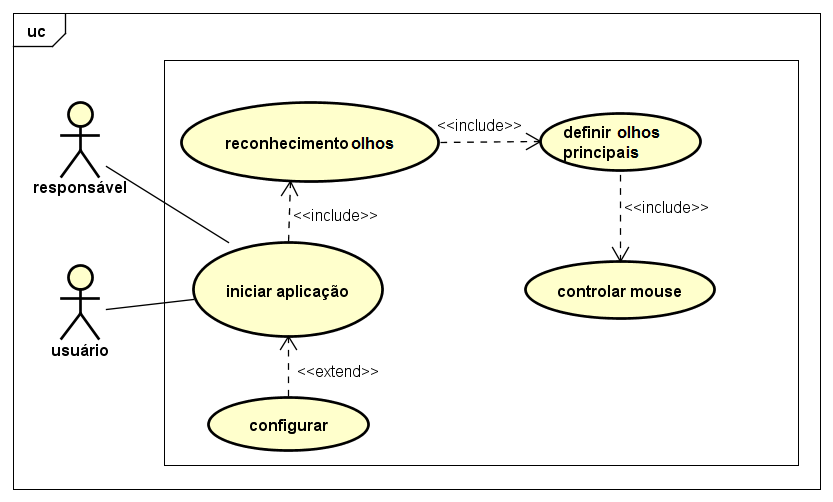
\includegraphics[scale=.5]{img/UseCase_Diagram_2.png}

{\fontsize{11}{11}\selectfont \textbf{Fonte:} Elaborada pelo autor.}
\label{fig:use-case-diagram}
\end{figure}

O início do funcionamento é marcado pela inicialização da aplicação, representado como a elipse “Iniciar aplicação” no diagrama. Em seguida é feito o reconhecimento dos olhos, representado pela elipse “Reconhecer olhos” no diagrama, a aplicação ainda define qual das duplas de olhos ele deve rastrear, esta funcionalidade é representada pela elipse “Definir olhos principais” no diagrama.  Após isto é dado o controle do \textit{mouse} para o usuário, é feita uma simulação do \textit{mouse}, representado pela elipse “Controlar mouse”, além disto é possível entrar na área de configuração a qualquer momento, representado pela elipse “Configurar”.


% \textbf{[RCC - O capítulo de modelagem, pra mim está mais para uma seção lá do teu desenvolvimento. São menos de 2 páginas, não vejo ele como um capítulo. Acredito que ajudaria puxar para uma seção dentro do capítulo de desenvolvimento. Tipo, tu define a arquitetura geral, e depois sai detalhando, ou modelando, a solução. Aí, até se encaixaria esses diagramas. Onde ele está posicionado atualmente, não me parece fazer muito sentido. Ou se move ele (e se ajusta o texto para fazer sentido), ou se retira. É o q eu faria...}]


\chapter{VISIUMOUSE}\label{CAP4}
VisiUMouse é um projeto de VC com o objetivo de ajudar pessoas com algum tipo de deficiência físico motora a utilizar o computador de maneira simples e fácil apenas com do movimento da cabeça, usando os olhos como referência. A ideia é permitir a substituição do \textit{mouse} convencional por uma nova IHC adequada e configurável. A técnica de  rastreamento dos olhos do usuário é sutil e não causa nenhum desconforto, para usuários que não podem usar dispositivos tradicionais de entrada de computador, como teclado e \textit{mouse}.

\section{Arquitetura}\label{Sub:funcionamento-visiumouse}
VisiUMouse é um projeto que tem como objetivo principal a utilização de computadores pessoais (PC) exclusivamente com o movimento da cabeça, isto é possível com base na captura de vídeo feita pelo \textit{webcam} do usuário e o processamento dos dados do vídeo recebidos, e com o uso de algoritmos de rastreamento de objetos e \textit{Machine Learning} é possível reconhecer a posição atual dos olhos do usuário. A Figura \ref{fig:projeto-diagrama-alto-nivel} apresenta um diagrama de alto nível do funcionamento do VisiUMouse. 

\begin{figure}[H]
\centering
\caption{Diagrama de alto nível do VisiUMouse.}
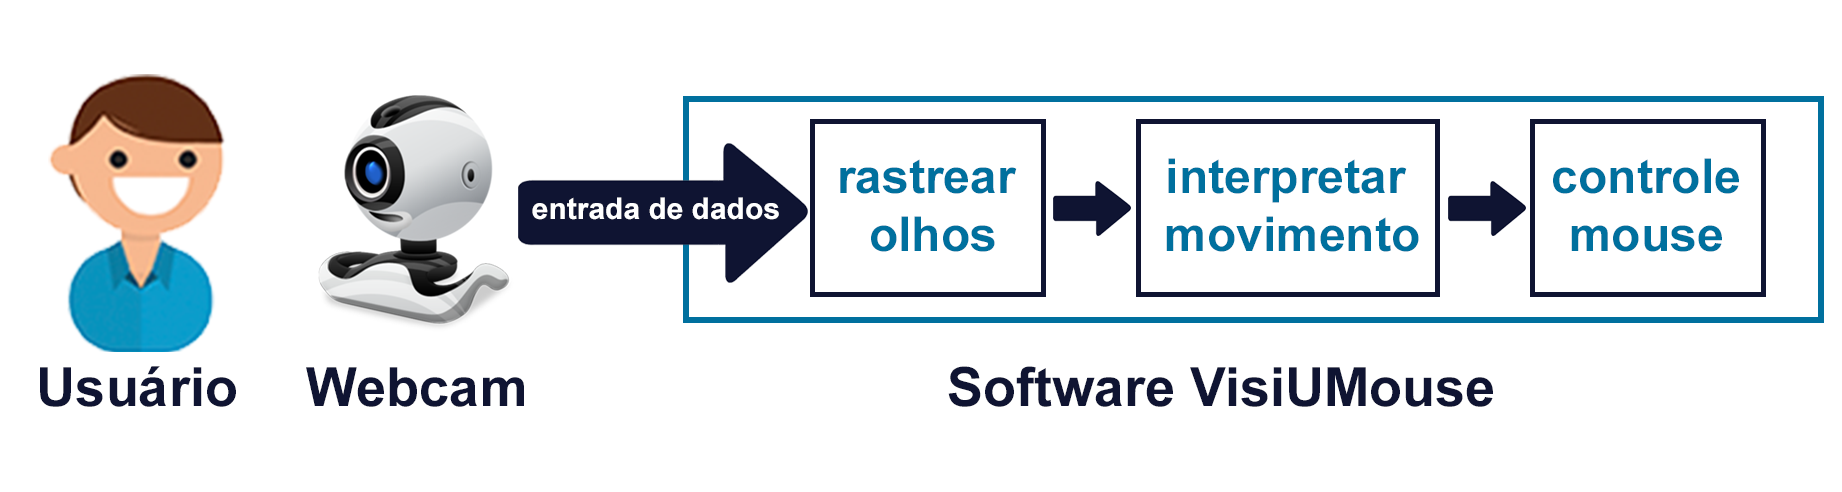
\includegraphics[scale=.23]{img/projeto-diagrama-alto-nivel.png}

{\fontsize{11}{11}\selectfont \textbf{Fonte:} Elaborada pelo autor.}
\label{fig:projeto-diagrama-alto-nivel}
\end{figure}


Do lado direito é possível ver o Usuário posicionado a frente da \textit{Webcam}, a qual é responsável por capturar vídeo deste Usuário. Para cada captura (ou \textit{frame}) do vídeo é enviado um conjunto de dados para o VisiUMouse, como entrada de dados que será processado pela aplicação. Após a leitura dos dados é iniciado o processo de rastreamento dos olhos, representado por 'rastrear olhos'. Em seguida ao rastreamento é feita uma análise que interpreta o movimento/deslocamento dos olhos do usuário, como podemos ver em 'interpretar movimento'. Por fim, o movimento dos olhos do usuário é retratado no controle do movimento do \textit{mouse}, representado por 'controle mouse'.


O processo de \textit{Machine Learning} é utilizado para reconhecer padrões de formas de objetos. Neste caso foi para rastrear olhos humanos, sendo  necessário utilizar um banco de dados com grande volume de imagens de olhos que gerou um arquivo XML com estes padrões. Com o arquivo XML que contêm os padrões foram utilizados os conceitos do algoritmo de Viola-Jones para fazer o processo de rastreamento \cite{viola2001rapid}. Este arquivo XML contém os padrões e características, denominados \textit{haar features}, que consistem em uma lista de padrões e características invariantes de um determinado objeto.

Os objetos procurados pela estrutura de detecção universalmente envolvem as somas de píxeis de imagem dentro de áreas retangulares. Estes valores são comparados com os valores dos estágios do arquivo \textit{haar features}, e assim determinar se a área examinada da imagem possui ou não o objeto que pretende detectar. A Figura \ref{fig:viola-jones-ret} apresenta o processo de somas de píxeis da imagem que está sendo trabalhada, as somas são feitas dentro dos retângulos. 

\begin{figure}[H]
\caption{Processo de somas de píxeis de uma imagem} 
\centering 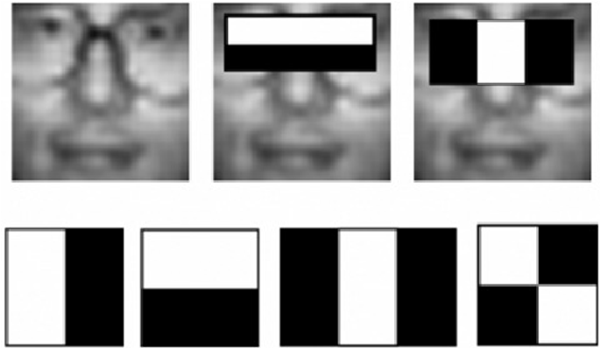
\includegraphics[scale=0.6]{img/viola-jones-ret.png}

{\fontsize{11}{11}\selectfont \textbf{Fonte:} Elaborada pelo autor.}
\label{fig:viola-jones-ret}
\end{figure}

Aplicação de rastreamento dos olhos foi desenvolvida usando a linguagem de programação Java, já que esta linguagem oferece um arsenal de bibliotecas para PDI e o suporte a desenvolvimento de sistemas multiplataforma, isto é, funciona em diferentes Sistemas Operacionais. 

Normalmente os processos de rastreamento são feitos em um processador responsável pela renderização de gráficos em tempo real. Este tipo de processador é chamado de \textit{Graphics Processing Unit}, ou GPU.

Genericamente o processamento da imagem contém 3 estágios: Captura, Análise e Compressão da Imagem. A \textbf{Captura} trata da aquisição dos dados de entrada de vídeo; a \textbf{Análise} trata do reconhecimento do objeto alvo. Para o reconhecimento é necessário um conjunto de padrões do alvo, esse processo é nomeado de Treinamento e é responsável por gerar um arquivo XML que contém características e padrões do objeto alvo. A Classificação é o processo final que define se um determinado pedaço da imagem contém o objeto que pretende detectar. A \textbf{Compressão da Imagem} é o processo feito para reduzir a redundância dos dados, de forma a armazenar ou transmitir esses mesmos dados de forma eficiente, de acordo com \citeonline{rolim2008sistema}.

Com os conceitos do algoritmo de Viola-Jones e as bibliotecas de suporte a PDI foi possível desenvolver o VisiUMouse, o qual tem como característica principal o reconhecimento e rastreio dos olhos do usuário, para  que ele controle o \textit{mouse}. O processo de movimento dos olhos e o movimento do ponteiro do \textit{mouse} é dado em dezenas de milissegundo, este valor depende da GPU do computador do usuário. A Figura \ref{fig:visiumouse-1} mostra o funcionamento do rastreando dos olhos do usuário.
\begin{figure}[H]
\centering
\caption{Tela de captura de vídeo do VisiUMouse.}
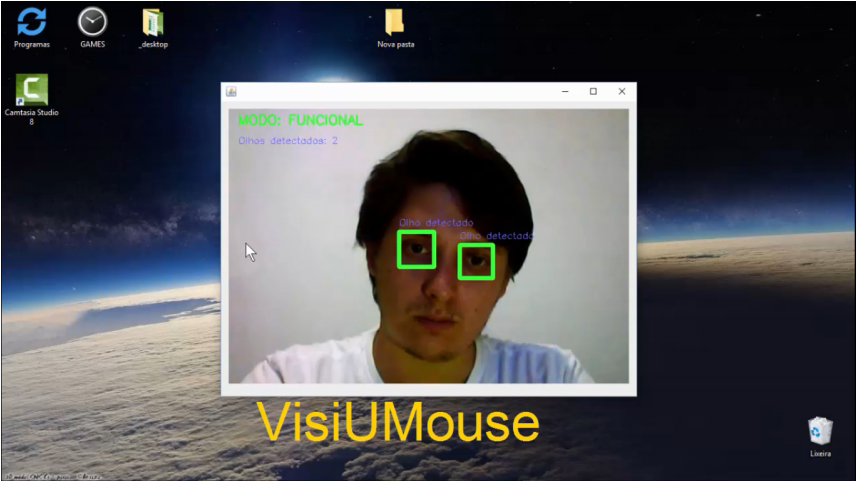
\includegraphics[scale=.4]{img/visiumouse-1.png}

 {\fontsize{11}{11}\selectfont \textbf{Fonte:} Elaborada pelo autor.}
\label{fig:visiumouse-1}
\end{figure}

O VisiUMouse tem seu funcionamento baseado no movimento da cabeça/face, usando os olhos como ponto de referência e a Técnica de Zona Neutra e de Movimento (TZNM). A medida do deslocamento dos olhos é feita através do processamento das posições anteriores, ou seja, se a medida for superior a configurada é feita a movimentação do ponteiro (zona de movimento da TZNM), se for menor o ponteiro permanece parado (zona neutra da TZNM). Para processar para qual lado o cursor deve ir é verificada a posição dos olhos em relação às linhas (ilusórias) vermelha e verde, como pode ser visto na Figura \ref{fig:funcionamento}.

\begin{figure}[H]
\caption{VisiUMouse: telas de rastreamento e processamento do deslocamento dos olhos.}
\centering 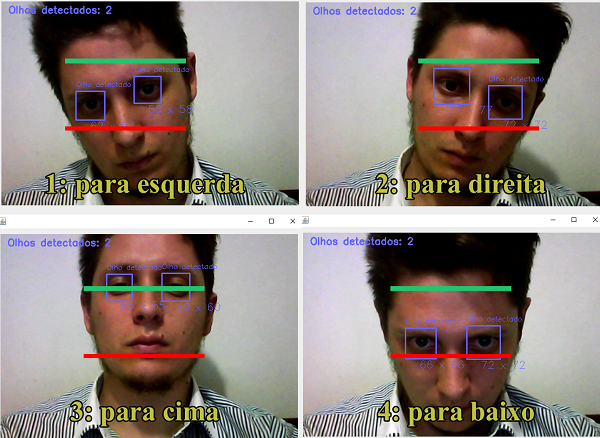
\includegraphics[scale=.8]{img/funcionamento2.png}

{\fontsize{11}{11}\selectfont \textbf{Fonte:} Elaborada pelo autor.}
\label{fig:funcionamento}
\end{figure}

Para determinar a direção do movimento do ponteiro é feita uma comparação com a posição dos olhos em relação às linhas verde e vermelha. Por exemplo, se o olho direito estiver próximo da linha verde e o olho esquerdo próximo da linha vermelha, indica que o usuário está com a cabeça inclinada para esquerda e que o cursor do \textit{mouse} deve ir para o mesmo lado, como mostrado na Figura \ref{fig:funcionamento} (1: para esquerda). Também é possível fazer movimentos para direita, para cima e para baixo (vide Figura \ref{fig:funcionamento}), além da combinação desses movimentos, tornando possível realizar movimentações em diagonal. No momento em que o movimento do cursor do \textit{mouse} se inicia, o usuário não precisa mais deslocar os olhos para manter o movimento, ele apenas precisa permanecer na mesma posição, podendo tornar o controle do \textit{mouse} menos cansativo, e assim evitando o desgaste físico do usuário \footnote{Foi disponibilizado um vídeo com o funcionamento básico do VisiUMouse, em: http://visiumouse.com/\#funcionamento}. 




%%ALIÁS, FARIA MUITO MAIS SENTIDO SE ESTAS OBSERVAÇÕES E A TABELA COMPARATIVA ESTIVESSE EM TRABALHOS RELACIONADOS
\subsection{Comparação com Soluções Análogas}\label{Sub:tabela-comparativa}
A área de TA apresenta um número significativo de tecnologias que permitem o melhor uso de um computador e comunicação, entra elas podemos citas as que utilizam poder computacional, como as que permite o uso do computador apenas com o movimento da cabeça, geralmente a leitura do movimento é feito por um  entrada de vídeo que filma e interpreta seus movimentos, as soluções apresentadas a seguir utilizam essas premissas.

A Tabela \ref{tabela-comparativa} apresenta uma comparação entre os \textit{softwares}: VisiUMouse, CameraMouse e FacialMouse; os quais apresentam algumas semelhanças como: \textit{webcam} como entrada de vídeo, uso da biblioteca OpenCV e do algoritmo de Viola-Jones. A Tabela \ref{tabela-comparativa} apresenta 6 atributos de comparação:

%https://www.tablesgenerator.com/
% Please add the following required packages to your document preamble:
% \usepackage[table,xcdraw]{xcolor}
% If you use beamer only pass "xcolor=table" option, i.e. \documentclass[xcolor=table]{beamer}
\begin{table}[H]
\centering
\caption{Tabela Comparativa dos Sistemas de TA baseados em vídeo}
\label{tabela-comparativa}
\begin{tabular}{|l|l|l|l|}
\hline
\multicolumn{1}{|c|}{\textbf{Tecnologia Assistiva}} & \multicolumn{1}{c|}{\textbf{VisiUMouse}} & \multicolumn{1}{c|}{\textbf{CameraMouse}} & \multicolumn{1}{c|}{\textbf{Facial Mouse}} \\ \hline
Clique por Tempo                                     & \cellcolor[HTML]{67FD9A}Sim              & \cellcolor[HTML]{67FD9A}Sim                & \cellcolor[HTML]{67FD9A}Sim                \\ \hline
Tipos  de Cliques                                    & Principais                               & Principais                                 & Esquerdo                                   \\ \hline
Multiplataforma                                     & \cellcolor[HTML]{67FD9A}Sim              & \cellcolor[HTML]{67FD9A}Sim                & \cellcolor[HTML]{67FD9A}Sim                \\ \hline
Tipo de Movimento                                   & TZNM                                     & Espelhado                                  & Espelhado                                  \\ \hline
Objeto Rastreado(s):                                & Olhos                                    & Selecionável                              & Rosto                                      \\ \hline
Quantidade de Objetos Rastreados:                   & 2                                        & 1                                          & 1                                          \\ \hline
\end{tabular}
\end{table}

\begin{enumerate}
\item \textbf{Clique por Tempo}: os dispositivos de TA com base em vídeo geralmente utilizam a técnica do clique do \textit{mouse} para simplificar o uso, esta técnica consiste em deixar o cursor do \textit{mouse} parado por um determinado tempo para gerar o clique na mesma posição que o curso está. Apesar de o clique por tempo ser comumente utilizado pode influenciar no desempenho do usuário em executar tarefas no computador que necessitam ser rápidas, como jogos. O VisiUMouse faz o rastreamento dos olhos permitindo implementar uma funcionalidade de clique pelo piscar dos olhos. 

\item \textbf{Tipos de Cliques}: este atributo representa a variedade de tipos de clique e funcionalidade do \textit{mouse} que a tecnologia apresenta, entre eles estão o clique primário (comumente o botão esquerdo do \textit{mouse}), clique secundário (comumente o botão direito do \textit{mouse}), a funcionalidade de arrastar etc.

\item \textbf{Multiplataforma}: característica de um sistema funcionar igualmente em diferentes plataformas (Sistemas Operacionais).

\item \textbf{Tipo de Movimento}: atributo que define como o movimento do cursor é feito em ralação ao objeto rastreado. As TA apresentadas utilizam o movimento espelhado que pode ser determinado por um reflexo do movimento do objeto rastreado no momento do cursor do \textit{mouse}, apesar de ser intuitivo pode causar um desgaste físico extra na região do pescoço e tornar inviável para pessoas que tenham menos mobilidade com a cabeça. A TZNM apresenta uma solução alternativa para o movimento do cursor do \textit{mouse} possibilitando um desgaste físico menor e o movimento por toda a tela do computador com uma menor mobilidade da parte do usuário.

\item \textbf{Objeto Rastreado(s)}: atributo que define qual objeto da cabeça do usuário é rastreado, ou seja, o objeto que o \textit{software} vai identificar a cada \textit{frame} da entrada de vídeo para definir o deslocamento desse objeto. O CameraMouse permite uma configuração de qual objeto vai ser rastreado, porém perde a referência com algum tempo de uso fazendo com que o usuário precise configurar de novo o objeto. Já o FacialMouse rastreia o rosto do usuário permitindo que o usuário não precise fazer uma configuração antes de usar. O VisiUMouse rastreia os 2 olhos do usuário possibilitando 2 pontos de referência que podem aumentar a precisão da leitura dos movimentos do usuário.

\item \textbf{Quantidade Objeto Rastreado(s)}: define a quantidade de objetos que sera rastreado, quanto maior a quantidade mais pontos de referencia a aplicação vai ter para entender o movimento do usuário.
\end{enumerate}

\section{Site}\label{sub:visiumouse-objtivo-site}
Além do \textit{software} do VisiUMouse foi desenvolvido um site com o objetivo de facilitar a disponibilização da solução, registrar os usuários do VisiUMouse e captar seus dados de contato. 
No site é disponibilizado o VisiUMouse para \textit{download}, o usuário tem acesso a todas as versões, além de ser capaz ver as características de cada versão e suas respectivas compatibilidades. O VisiUMouse é disponibilizado no formato de um instalador, que facilita a instalação no computador do usuário. A Figura \ref{fig:site-download} mostra a página no site que o usuário acesso para fazer o \textit{download} do VisiUMouse.


\begin{figure}[H]
\caption{Página de downloads do site.} 
\centering 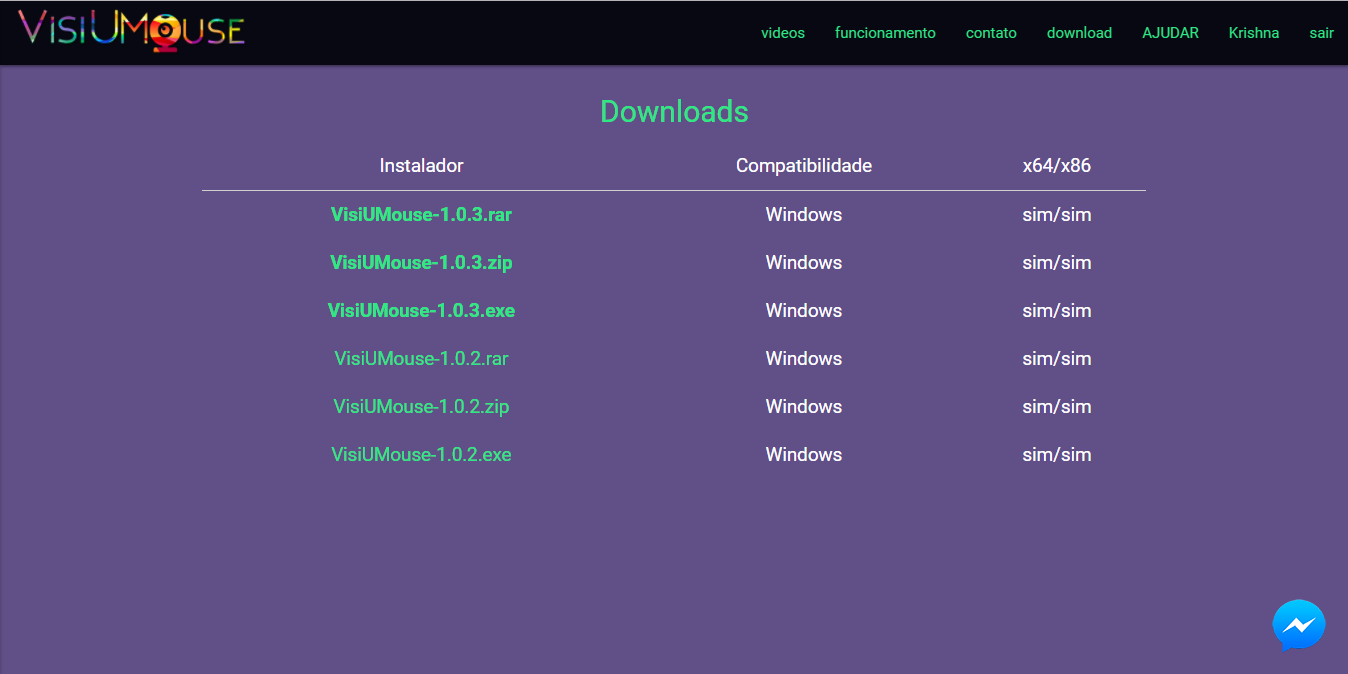
\includegraphics[scale=0.35]{img/site-download.png}

{\fontsize{11}{11}\selectfont \textbf{Fonte:} Elaborada pelo autor.}
\label{fig:site-download}
\end{figure}



\section{DESIGN}\label{CAP6}

A importância do Design está no desenvolvimento de produtos (digitais ou físicos). O Design pode dar destaque a um produto com as mesmas funcionalidades e preço de outro produto. Assim como um Design bem pensado desperta o desejo dos consumidores, um Design pobre e mal feito gera uma repulsa enorme \cite{patterson2017computer}.

Este seção destaca o Design da Interface e do site do VisiUMouse. O VisiUMouse é uma tecnologia \textit{desktop} executada pelo usuário na área de trabalho do computador, permitindo que ele controle o computador; o site é o responsável por apresentar e disponibilizar o VisiUMouse na \textit{Web} para os usuários, entre outras funcionalidades.

\subsection{Design da Interface Desenvolvida}\label{Sub:software}
Para a criação da interface foram utilizados os conceitos de CRAP (Contraste, Repetição, Alinhamento e Proximidade),de acordo com \citeonline{williams2005design}. A escolha da paleta de cores foi definida através de um levantamento das principais cores das tecnologias digitais atuais, foi feito uma pequena alteração nesta paleta para torná-la única e por consequência uma característica da própria tecnologia, as outras estilizações como sombra e tipografia foram definidas através das tendências atuais. Além de seguir boas práticas de \textit{Graphical User Interface} (GUI) para pessoas com pouca mobilidade, por exemplo botões grandes e mais afastados. A Figura \ref{fig:interface-tecnologia} mostra a tela principal do \textit{software} VisiUMouse.

\begin{figure}[htbp]
\caption{Interface principal do VisiUMouse.} 
\centering 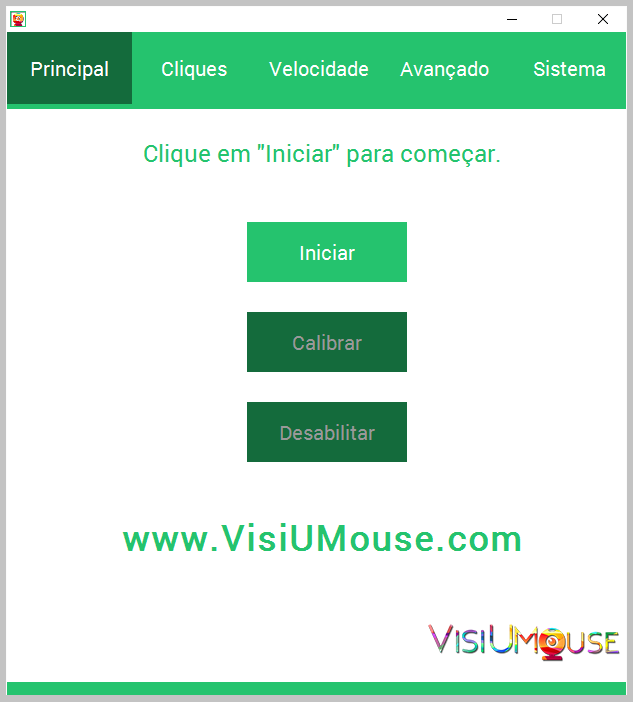
\includegraphics[scale=.5]{img/visiumouse-tela-principal-v216.png}

{\fontsize{11}{11}\selectfont \textbf{Fonte:} Elaborada pelo autor.}
\label{fig:interface-tecnologia}
\end{figure}

\subsection{Design do Site}\label{Sub:site}

O desenvolvimento do site tem como objetivo disponibilizar todo o conteúdo referente ao VisiUMouse, como o próprio \textit{software}, informações, módulos que foram criados juntamento com o VisiUMouse, uma página de contato entre outros. A Figura \ref{fig:site} apresenta a página inicial do site, no topo esta presente o menu de navegação que é fixo que permite que o usuário navegue entre todo o site de forma simples.

\begin{enumerate}
\item \textit{Inicial}: esta representado como a logo do site, do lado extremo esquerdo, ao clicar nessa imagem o usuário volta para o inicio da página;

\item \textit{Vídeos}: essa seção mostra um conjunto de vídeos que tem como objetivo dar uma visão geral do VisiUMouse;

\item \textit{Funcionamento}: apresenta uma explicação resumida de como utilizar o VisiUMouse;

\item \textit{Contato}: nessa seção é possível enviar uma mensagem para os idealizadores da solução VisiUMouse.
\end{enumerate}


\begin{figure}[htbp]
\caption{Interface da página inicial do Site.} 
\centering 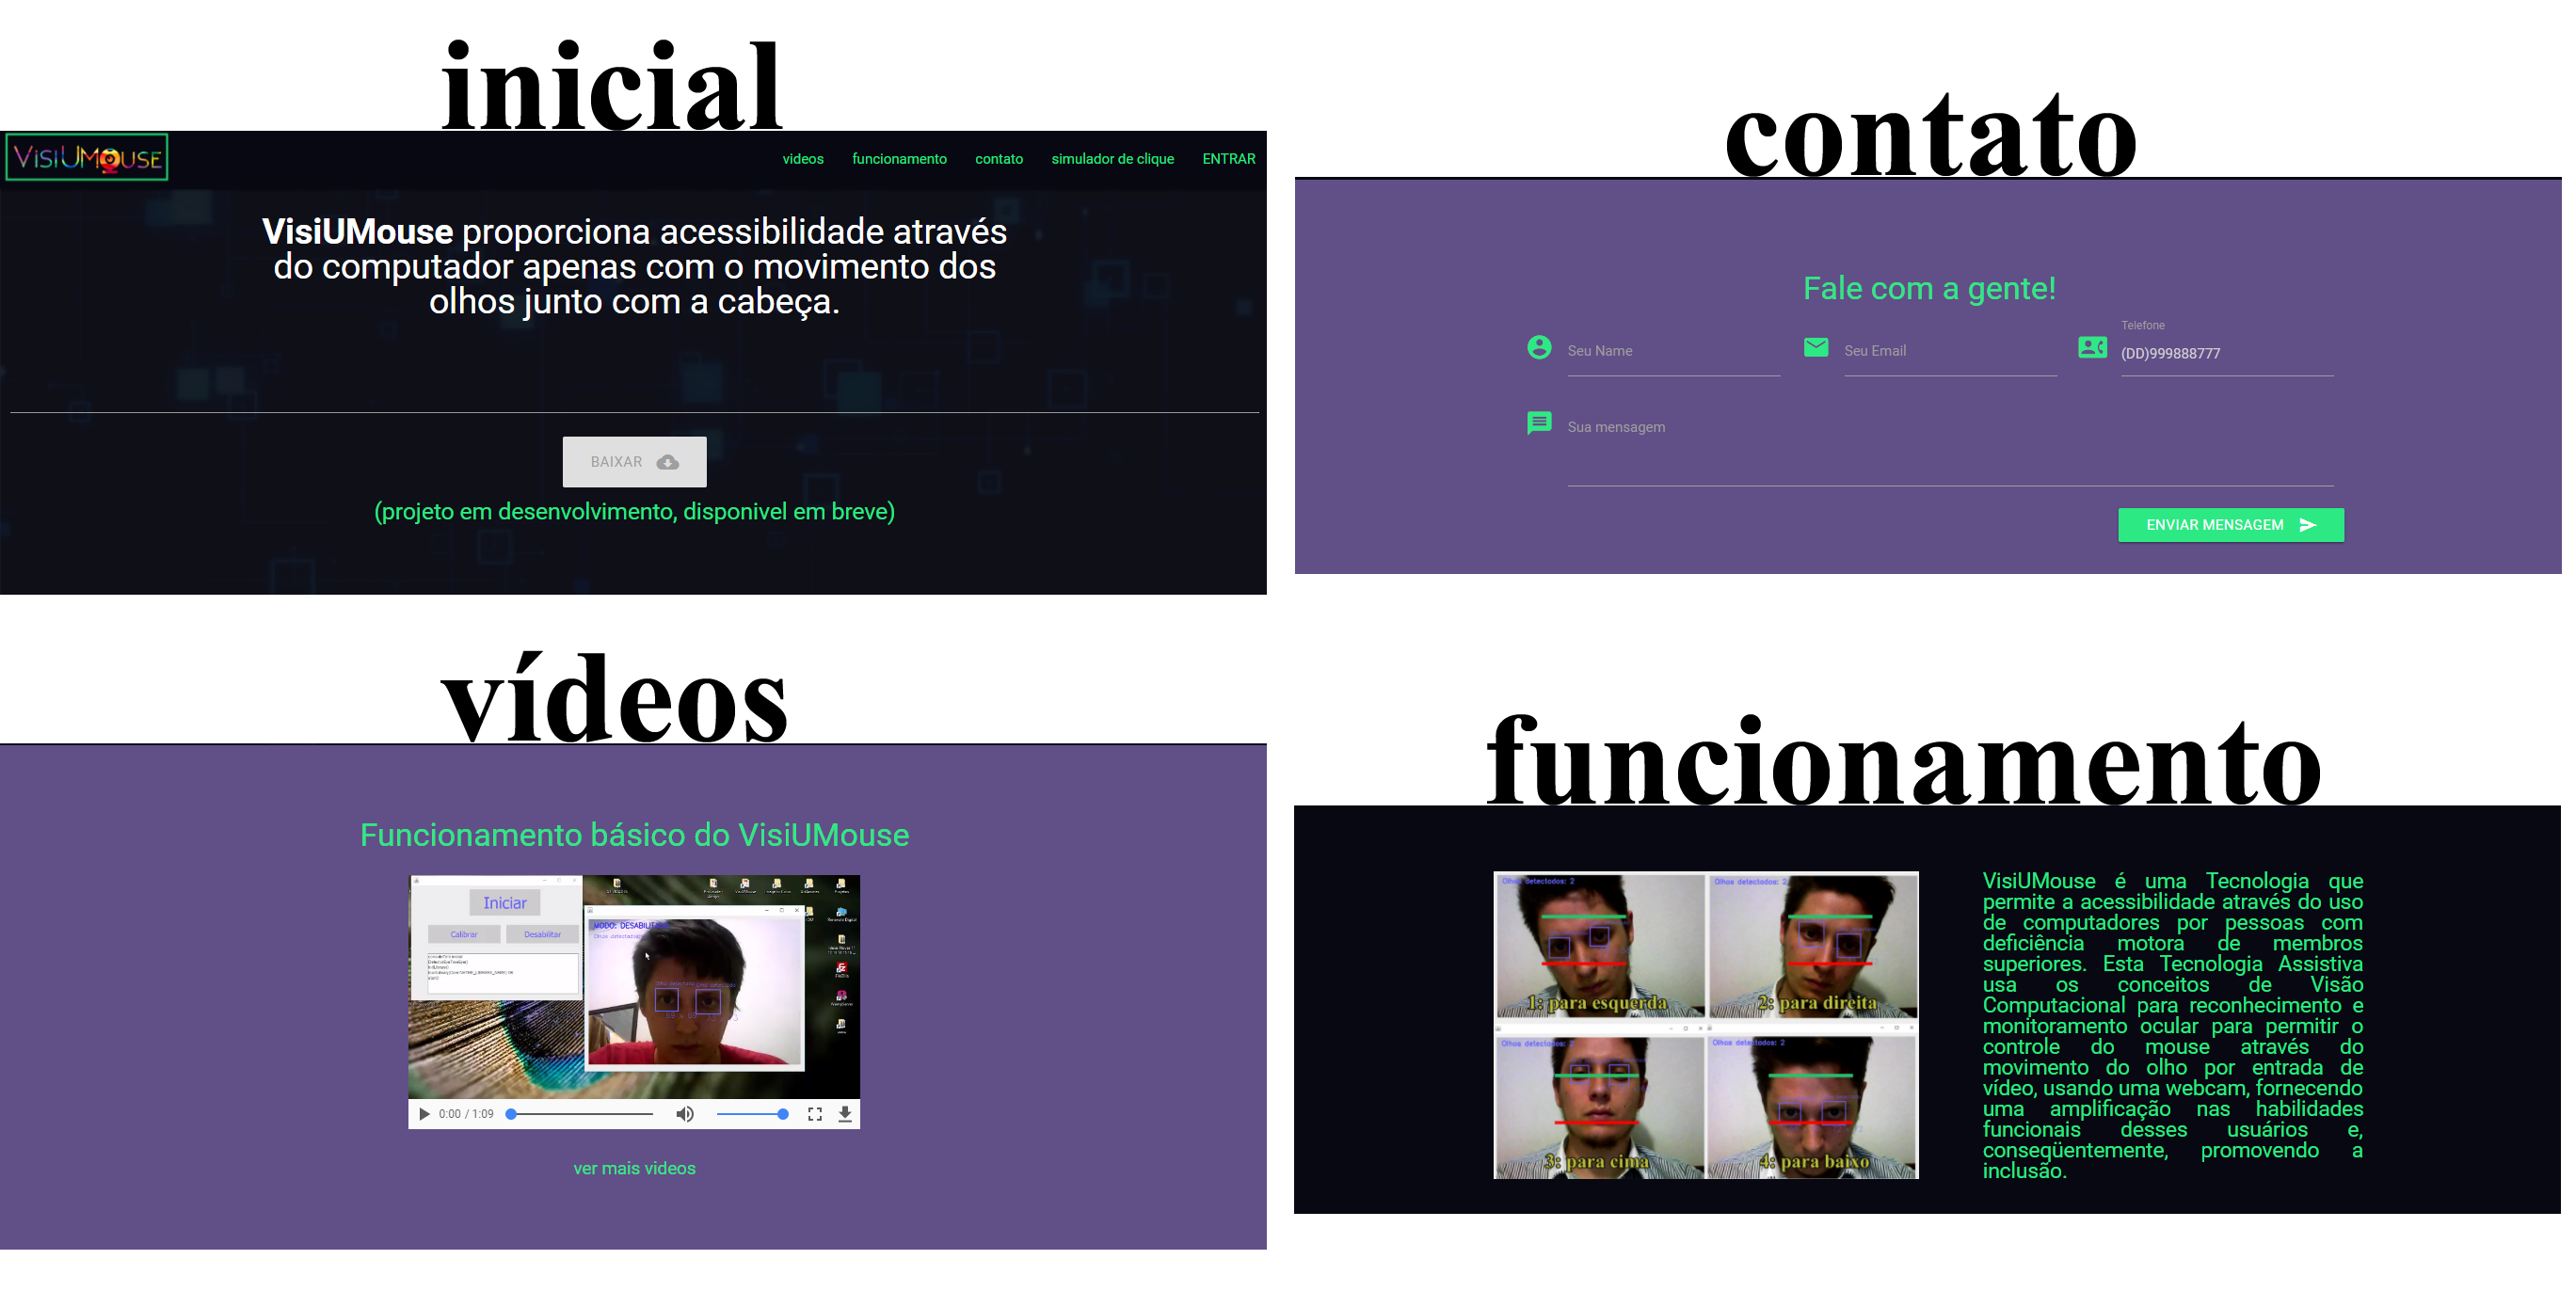
\includegraphics[scale=.33]{img/site.png}

{\fontsize{11}{11}\selectfont \textbf{Fonte:} Elaborada pelo autor.}
\label{fig:site}
\end{figure}

\chapter{TECNOLOGIAS UTILIZADAS}\label{CAP6-tecnilogias-utilizadas}
Neste capítulo, serão apresentadas as tecnologias utilizadas e desenvolvidas nesse trabalho, por questão de organização será segmentando 2 partes, as tecnologias utilizadas no software e site.

\section{Desenvolvimento do Software Desktop}\label{Sub:tecnologias-software}

A principal tecnologia utilizada foi a linguagem de programação Java, entre suas principais características está a possibilidade do desenvolvimento multiplataforma, permitindo que um mesmo \textit{software} seja executado em diferentes Sistemas Operacionai. Também foram utilizados a linguagem de programação C e a biblioteca OpenCV. A linguagem C foi responsável pelos algoritmos de processamento de imagens, por se tratar de uma tecnologia de baixo nível ela apresenta uma alta eficácia no processamento de dados, essa característica é de extrema importância em soluções que precisam de um alto poder computacional.

Para o desenvolvimento do \textit{software} VisiUMouse foi criado um conjunto de ferramentas para auxiliar, como um Simulador de \textit{Mouse}; um \textit{script} para otimizar o controle de versões, o \textit{Auto Commit} e um protocolo para metrificar testes, o Fitts Task Two, os quais estão presentes nos tópicos seguintes.

\subsection{Linguagem de Programação Java}

Criada pela equipe de desenvolvedores liderada por James Gosling na Sun Microsystems (atualmente de propriedade da Oracle) e lançada em 1995, o Java é uma linguagem de programação Orientada a Objetos que atualmente faz parte do núcleo da plataforma Java. A Orientação a Objetos, ou Programação Orientada a Objetos (POO), é um paradigma de análise, para a programação de sistemas no qual todos os elementos inseridos são objetos \cite{urma2014java}.

A linguagem Java possui arquitetura neutra e portável, de forma que pode ser utilizada em diversos Sistemas Operacionais, ter alta performance, apresentar segurança e solidez e ser uma linguagem interpretada com suporte a \textit{threads} e dinâmica. As aplicações em Java normalmente podem ser executadas em qualquer plataforma que possua a \textit{Java Virtual Machine} (JVM) instalada, independente da arquitetura do computador.

Entre os pontos que justificam a escolha da plataforma Java, podemos destacar: o alto nível de compatibilidade com diferentes plataformas, alto desempenho, solidez e compatibilidade com a biblioteca OpenCV.

\subsection{Linguagem de Programação C}

A linguagem C foi criada por Dennis Ritchie em 1972 com um propósito: ser usada no desenvolvimento de uma nova versão do sistema operacional Unix. C é capaz de gerar programas extremamente rápidos em tempo de execução, possui uma sintaxe simples e poderosa, com instruções de alto nível. A linguagem C influenciou de forma direta muitas linguagens como C++, Java, C\# , Objective C, e muitas outras linguagens de programação tem sua sintaxe e estruturas influenciadas por C, segundo \citeonline{backes2012linguagem}.

Entre suas características principais podem citar: a Portabilidade, geração de códigos executáveis compactos e rápidos, interação com o Sistema Operacional e linguagem estruturada. A geração de códigos compactos e rápido ganha destaque nos algoritmos de PDI.

Entre os pontos que justificam a escolha da linguagem C, podemos destacar: alto poder de processamento, interação com o Sistema Operacional e compatibilidade com a biblioteca OpenCV.

\subsection{OpenCV}

O OpenCV (\textit{Open Source Computer Vision Library}) é uma biblioteca multiplataforma desenvolvida pela Intel Corporation, que implementa diversos módulos para VC, este os quais são utilizados para o Processamento de Imagens e Vídeo, Estruturas de dados, álgebra linear e mais de 350 algoritmos de VC. OpenCV possui, em seu módulo central uma implementação do algoritmo de Viola-Jones para detecção de objetos, de acordo com \cite{bradski2008learning}.

\subsection{Simulador de Mouse}

O Simulador\footnote{O Simulador está disponível em: https://github.com/KrishnaXavier/system-click-time} é uma aplicação capaz de simular um \textit{mouse} comum, com o clique com base no tempo, isto é o clique é gerado após um determinado tempo parado, esse tempo pode ser configurado, além disso ele também simula os principais cliques de um \textit{mouse}, como o clique do botão primário (geralmente é representado pelo botão esquerdo do \textit{mouse}), duplo primário, botão secundário (geralmente é representado pelo botão direito do \textit{mouse}) e a função de arrastar. Ele possibilita manter as métricas do clique igual para testes comparativos entre diferentes dispositivos, como o experimento descrito no Capítulo \ref{CAP7}, que apresenta um teste de comparação do VisiUMouse com o \textit{mouse} tradicional.


\subsection{\textit{Fitts Task Two}}

O Fitts Task Two\footnote{O Protocolo está disponível em: https://github.com/KrishnaXavier/FittsTaskTwo} é um protocolo baseado na Lei de Fitts, proposto por \citeonline{soukoreff2004towards}. Ele permite metrificar o ato de 'apontar' na movimentação humana, como o controle \textit{mouse}. A aplicação desenvolvida foi criada a partir do protocolo Fiits Task Two, boa parte do código foi mantida, foram feitas apenas altercações necessárias para realizar o experimento descrito no Capítulo \ref{CAP7}.

\subsection{Auto Commit}

O Auto Commit\footnote{O Auto Commit está disponível em: https://github.com/KrishnaXavier/auto-commit} é uma sequência de comandos implementados em um \textit{software} executável, ou seja, um \textit{script}, que permite salvar as alterações de qualquer aplicação de forma mais amigável, apenas com um comando. Esse \textit{script} foi criando visando ajudar os desenvolvedores que tem dificuldade em salvar as alterações das suas aplicações.



\section{Tecnologias utilizadas na criação do Site}\label{Sub:tecnologias-site}
As tecnologias utilizados no desenvolvimento do site foram divididas em 2 categorias, as que funcionam no lado do servidor (\textit{Server-side}) e as que funcionam apenas no lado do cliente (\textit{Client-side}). Entre as tecnologias \textit{Server-side} podemos citar o PHP e MySQL. E entre as tecnologias \textit{Client-side} podemos citar HTML5, CSS, JavaScript, \textit{Framework }JQuery e \textit{Framework} Materialize. Além disso foram utilizadas as arquiteturas MVC e SPA. Para a criação da estrutura do PHP Orientado a Objetos foi desenvolvido uma ferramenta, o Creator OOP Structure.

A escolha das tecnologias para o desenvolvimento do site se deu pelo fato de serem tecnologias consagradas na área de desenvolvimento web. Todas elas dispõe de um acervo grande de documentação e livros, além de contar com constantes atualizações e melhorias.

\subsection{PHP 5}

A linguagem de programação PHP (um acrônimo recursivo para \textit{PHP: Hypertext Preprocessor}) é uma linguagem de \textit{script} de código aberto de uso geral, muito utilizada, e especialmente adequada para o desenvolvimento web e que pode ser embutida dentro do HTML. Ela frequentemente é utilizada para a comunicação com o Banco de Dados. A linguagem permite que se adicione dinamicidade aos projetos web, ou seja, o conteúdo da página é montado durante a requisição e então enviado ao cliente, segundo \citeonline{converse2003php}.

\subsection{MySQL}

O sistema MySQL foi desenvolvido pela empresa sueca MySQL AB e publicado, originalmente, em maio de 1995. O MySQL é um sistema de gerenciamento de banco de dados (SGBD) de código aberto, que utiliza a linguagem SQL (\textit{Structured Query Language}) como interface. É atualmente um dos sistemas de gerenciamento de Bancos de Dados mais populares, com mais de 10 milhões de instalações pelo mundo, de acordo com \citeonline{miletto2014desenvolvimento}.

\subsection{HTML5}

Como \citeonline{silva2015fundamentos} define, o HTML (\textit{HyperText Markup Language}, que significa Linguagem de Marcação de Hipertexto) é uma linguagem de marcação utilizada na construção de páginas na Web. Documentos HTML podem ser interpretados por navegadores. A tecnologia é fruto da junção entre os padrões HyTime e SGML. Atualmente sua versão é a 5.0.

\subsection{CSS3}

CSS3 é a segunda mais nova versão das famosas \textit{Cascading Style Sheets} (ou simplesmente CSS), onde se define estilos para páginas web com efeitos de transição, imagem e outros, que dão um estilo novo às páginas Web em todos os aspectos de design do layout. CSS3 ultrapassou o status de proposta de uma tecnologia que prometia revolucionar a forma como estilizamos documentos para a web e deve obrigatoriamente fazer parte do dia a dia dos designers e desenvolvedores web, segundo \citeonline{silva2011css3}.

\subsection{JavaScript}

JavaScript é uma linguagem de programação interpretada que foi originalmente implementada como parte dos navegadores Web para que \textit{scripts} pudessem ser executados do lado do cliente e interagissem com o usuário sem a necessidade deste \textit{script} passar pelo \textit{Server-side}, controlando o navegador, realizando comunicação assíncrona e alterando o conteúdo do documento exibido. \cite{flanagan2007javascript-UPPERCASE}.

\subsection{Framework Materialize}

Materialize é um \textit{framework} \textit{Client-side} que resolve os mesmos problemas como alinhamento de objetos HTML e Desgin Responsivo. Ele surgiu através de um projeto desenvolvido pela Google e é inspirado no Material Design (design utilizado no sistema operacional para \textit{smartphones} Android desde a versão 5.0).

\subsection{Framework {j}Query}

O \textit{Framework} jQuery em JavaScript permite a abstração de tarefas comuns do \textit{Client-side}, como a manipulação de elementos da página, gerenciamento de eventos, requisições e Ajax. O jQuery permitiu uma codificação rápida e direta, diminuindo o código e o tornando mais legível, o que consequentemente tornou o desenvolvimento mais eficiente, \cite{duckett2018javascript}. Com o Ajax é possível implementar a arquitetura SPA, que esta descrita no tópico seguinte.

\subsection{Arquitetura SPA}

Um aplicativo de página única (\textit{Single Page Application}, ou SPA) é uma aplicação web ou site que consiste de uma única página web com o objetivo de fornecer uma experiência do usuário similar à de um aplicativo desktop. Em uma SPA, todo o código necessário - HTML, JavaScript, e CSS – ou é obtido com um único carregamento de página, ou os recursos apropriados são carregados dinamicamente e adicionados à página conforme necessário, geralmente em resposta a ações do usuário. A página não é recarregada em qualquer momento do processo, tampouco ocorre a transferência de controle para outra página. Interação com aplicativos de página única muitas vezes envolve comunicação dinâmica com o servidor web por trás dos bastidores, de acordo com \citeonline{mikowski2013single}.

\subsection{Arquitetura MVC}

Segundo \citeonline{teruel2012arquitetura} a arquitetura MVC é padrão de \textit{software} que permite dividir a aplicação em 3 camadas, \textit{Model}, \textit{View} e \textit{Controller}. O \textit{Model} consiste nos dados da aplicação, regras de negócios, lógica e funções. Uma \textit{View} pode ser qualquer saída de representação dos dados, como uma tabela ou um diagrama. É possível ter várias visões do mesmo dado, como um gráfico de barras para gerenciamento e uma visão tabular para contadores. O \textit{Controller} faz a mediação da entrada, convertendo-a em comandos para o \textit{Model} ou \textit{View}. As ideias centrais por trás do MVC são a reusabilidade de código e separação de conceitos.

\subsection{Creator OOP Structure}

Creator OOP Structure\footnote{O Creator OOP Structure está disponível em: https://github.com/KrishnaXavier/creator-oop-structure}  é uma ferramenta que auxilia a criação da estrutura do PHP Orientado a Objetos de forma a deixar a codificação mais rápida, para criar toda a estrutura ele apenas precisa do nome da classe, os seus atributos e as respectivas visibilidades.

\section{Controle de Versões}
Controle de Versões ou Sistema de Controle de Versões (ou ainda \textit{Control Version System}, {CVS}) é o processo pelo o qual um \textit{software} (seja um site ou aplicação \textit{desktop}) pode manter todo o histórico de alterações, seja uma pequena alteração como um correção ou melhoria ou uma grande alteração como a criação de uma nova funcionalidade, além de salvar quem e quando foi feita cada alteração. Outro ponto importante é que CVS permite o controle complexo de versões, ou seja, é possível desenhar todo o fluxo de desenvolvimento. 

Para o processo de CVS do VisiUMouse (site e aplicação \textit{desktop}) foi utilizado a ferramenta Git, que é uma tecnologia que permite o CVS de forma simples e prática, e como repositório do versionamento foi utilizado o GitHub. O GitHub é o maior repositório de \textit{software} de código aberto do mundo.



\chapter{AVALIAÇÃO}\label{CAP7}
% Dissertação do vinicius: https://www.overleaf.com/read/gbykffbhwqtk#/42933380/
% Capitulo 4 fala sobre os testes
A avaliação teve como objetivo fazer uma analise para determinar se o VisiUMouse é uma tecnologia que permite o controle do computador, para isso o VisiUMouse foi comparado com o \textit{mouse} tradicional. A comparação com o \textit{mouse} se da pelo fato de que atualmente os computadores utilizam-se dele como uma das principais ferramente de controle/interação.

% FALAR DO PERFIL DOS TESTERS
O experimento foi executado por 9 participantes voluntário, com idade média de 23,3 anos, alunos e professores do Instituto Federal Sul-rio-grandense Pelotas (IFSul) e entre eles 3 eram mulheres e 6 homens. Com o objetivo de fazer uma avaliação comparativa do \textit{software} VisiUMouse com o \textit{mouse} convencional para avaliar o seu funcionamento e objetivo principal. Para tanto foi utilizado um protocolo baseado na lei de Fitts, proposto por \citeonline{soukoreff2004towards}, envolvendo tarefas comuns como apontar, selecionar e clicar, que são usadas como métricas para verificar a interação com o computador. O protocolo foi configurado para 6 etapas, com 5 alvos cada, podendo ter o tamanho de 120, 150 ou 180 píxeis. O tamanho (gerados aleatoriamente) de cada um dos 5 alvos são iguais para cada fase \footnote{Foi disponibilizado gravações dos testes em: http://visiumouse.com}.

O teste foi dividido em 3 etapas: a primeira consistiu na aprendizagem de uso da aplicação, onde o participante era familiarizado com o funcionamento do VisiUMouse durante 5 minutos; a segunda etapa consistiu no experimento em si com o VisiUMouse; na última etapa, o participante utilizou o \textit{mouse} convencional para a execução das mesmas tarefas da etapa anterior. Os resultados são computados pelo \textit{software} do protocolo.

Para as três etapas foi utilizado o clique por tempo, ou seja, 
o clique é gerado depois de 5 segundos com o cursor do \textit{mouse} na mesma posição. Cabe ressaltar que em paralelo ao desenvolvimento do VisiUMouse foi criado um \textit{software} de clique por tempo para ser usado nos testes\footnote{Software de clique por tempo. Disponível em: http://visiumouse.com}. As demais configurações do VisiUMouse como velocidade foram mantidas iguais em todos os testes.  

O experimento foi conduzido com um notebook (LG S460) equipado com Windows 10, processador 2,4GHz (i3), 4 GB RAM, monitor de 14 polegadas, resolução de 1366 x 768 píxeis e utilizou-se a \textit{webcam} do próprio computador.

O interesse do experimento é em nível de protótipo, para tentar garantir que o desenvolvimento está no caminho certo, e para avaliar se o produto final atende ao público-alvo, porém quando se trata de pessoas com deficiência motora, no primeiro momento é necessário uma rodada de testes com pessoas sem nenhuma deficiência, conforme \cite{stone2005user}, para que os testes com o público-alvo já estejam cuidadosamente planejados e refinados. Além de buscar, com os profissionais da área de Terapia Ocupacional, conforme \cite{oliveira2015uso}, aspectos multidisciplinares relacionados a prescrição, habilidades e necessidades dos usuários.

\section{Resultados alcançados}\label{Sub:resultados-ex-1}
A Figura \ref{fig:assertividade} apresenta o gráfico dos resultados da assertividade dos cliques nos alvos. O software VisiUMouse (VUM, em azul) teve assertividade média de 99,63\%, representando apenas um erro com o participante 8. O \textit{mouse} comum (Mouse, em laranja) teve assertividade de 100\%, que já era esperado devido a grande familiaridade que os usuários já tinham com este dispositivo.

\begin{figure}[H]
\caption{Resultados da assertividade dos cliques nos alvos.} 
\centering 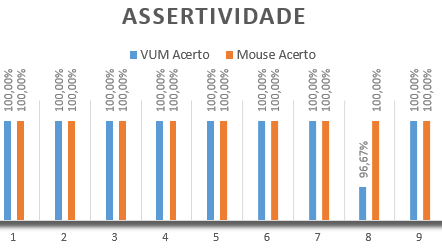
\includegraphics[scale=1]{img/assertividade.png}

{\fontsize{11}{11}\selectfont \textbf{Fonte:} Elaborada pelo autor.}
\label{fig:assertividade}
\end{figure}

A Figura \ref{fig:tmc} apresenta o gráfico com os resultados do tempo médio de cada clique (TMC), em milissegundos. O TMC do \textit{mouse} comum foi de aproximadamente 6372,4 milissegundos. O VisiUMouse (VUM) teve o TMC de aproximadamente 16579,5 milissegundos.
\begin{figure}[H]
\caption{Resultados do teste comparativo.} 
\centering 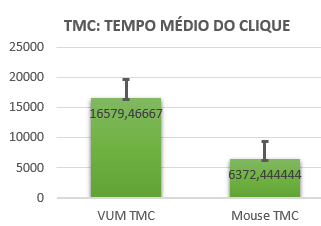
\includegraphics[scale=1]{img/tmc2.png}

{\fontsize{11}{11}\selectfont \textbf{Fonte:} Elaborada pelo autor.}
\label{fig:tmc}
\end{figure}

\section{Conclusões}\label{Sub:conclusao-ex-1}

A avaliação teve como proposito analisar o VisiUMouse, fazendo um comparação de assertividade e TMC em relação ao \textit{mouse} tradicional. A escolha da comparação com o \textit{mouse} se deu pelo fato de que ele é uma das principais ferramentas de interação com o computador.

A assertividade alcançada de 99,63\% do VisiUMouse indica seu potencial como uma alternativa substituta para o \textit{mouse} tradicional para pessoas com deficiência física nos membros superiores, o alto coeficiente de assertividade sugere uma alta precisão, mesmo para usuários que tiveram apenas 5 minutos de uso com a tecnologia.

Em contra ponto o TMC foi cerca de 10 segundos maior, isso indica que para interações mais ágeis pode haver dificuldades, tendo em vista a atenuação do TMC foi proposto mais configurações, as quais estão presente na versão atual do VisiUMouse, e como trabalho futuro o clique pelo piscar dos olhos.

Além disso a avaliação apontou a TZNM como um método favorável para o controle do movimento do \textit{mouse} em relação aos olhos do usuário, proposto em \cite{xavier2017visiumouse}.


\chapter{Conclusões}\label{CAP-consideracoes-finais-trabalhos-futuros}
Neste trabalho apresentou-se o desenvolvimento do VisiUMouse, que é uma tecnologia que permite o uso do computador para pessoas com deficiência física, para isso é feito o rastreamento dos olhos do usuário e convertido seus movimentos no movimento do cursor do \textit{mouse}, além disso o VisiUMouse permite vários tipos de cliques. O VisiUMouse apresenta uma interface de configuração simples e prática, que proporciona ajustes para melhor adaptação do usuário. Atualmente o VisiUMouse está na versão 1.2.6 e acessível para qualquer pessoa.

Tendo em vista os objetivos alcançado, como: \textbf{desenvolver uma TA com base em VC (objetivo principal)}, \textbf{desenvolver um site}, \textbf{criar um instalador}, \textbf{garantir que o VisiUMouse tenha as principais funcionalidades de um \textit{mouse}} e \textbf{criar uma interface de configuração amigável e de utilização simples} e os resultados da avaliação é possível indicar que o trabalho esta no caminho correto, uma vez que a solução ficou dentro do desejado, porém ainda existem melhorias a serem feitas.

\section{Trabalhos Futuros}

Entre os trabalhos futuros estão a implementação do rastreamento da visão, para os usuários que não tem a movimentação da cabeça; a implementação de uma aplicação para dispositivos móveis (celulares e \textit{tablets}) com as mesmas funcionalidades do VisiUMouse; e uma versão do VisiUMouse para macOS (Sistema Operacional da Apple); e a funcionalidade de clique pelo piscar dos olhos.

\begin{comment}

\end{comment}